\clearpage
\phantomsection
\section*{前言}\label{sec:preface}

最优传输的历史始于1781年Gaspard Monge提交给法国科学院的一篇论文\cite{ref231}. 此后，它发展成为一个成熟的数学领域，产生了许多重要发现，例如Kantorovich对偶理论、Brenier定理、Otto微积分、JKO格式，以及Lott--Sturm--Villani对测地空间Ricci曲率的定义等. 最早系统论述最优传输的是Rachev与Rüschendorf的开创性著作\cite{ref267,ref268}. 若希望从数学角度全面了解这一主题，还可参阅Villani\cite{ref315,ref317}、Ambrosio等人\cite{ref18}以及较近的Santambrogio\cite{ref281}的优秀教材；若希望快速入门，可阅读Ambrosio与Gigli的讲义\cite{ref17}、Ambrosio等人的讲义\cite{ref20}，以及Figalli与Glaudo的短篇专著\cite{ref133}. 即便只是粗略浏览这些书的目录，也能看出Monge的问题引出了许多后续问题，并且最优传输领域与从几何到偏微分方程的诸多方向都有出人意料的联系.

近年来，在Marco Cuturi的推动下，最优传输强势进入机器学习领域；他说明了可以用Sinkhorn算法高效计算Wasserstein距离\cite{ref97}. 最初的火花随后促成了一套广泛的工具，它们以最优传输为基础，涵盖机器学习与图形学各个领域的多种任务. 这套如今称为计算最优传输（computational optimal transport）的工具体系由Marco Cuturi和Gabriel Peyré引领发展，并汇集于他们富有启发性的专著\cite{ref257}. 最优传输在机器学习与数据科学中具有广泛用途，其基础在于点云、多边形网格，甚至文档等许多对象都能编码为概率测度；这些概率测度之间的Wasserstein度量于是提供了一种在语义上有意义的距离概念.

那么，什么是统计最优传输（statistical optimal transport）？这一修饰语主要呼应Peyré与Cuturi的计算最优传输. 它是一个总称，涵盖统计学与最优传输之间极其丰富多样的交汇点. 本专著旨在按照我们的兴趣，对这一蓬勃发展领域中的若干主题作入门介绍；互补的论述见\cite{ref253}.

历史上，Wasserstein距离一直是统计学中量化经验概率测度$\mu_n$向其极限$\mu$收敛速率的工具. 这一研究方向始于Dudley的著名工作\cite{ref121}，他给出了$W_1(\mu_n,\mu)$的界. Wasserstein距离尤其适合量化这种收敛，原因有几方面. 首先，与全变差距离或Kullback--Leibler散度不同，离散分布$\mu_n$与可能连续的分布$\mu$之间的Wasserstein距离仍然有限，且富含信息. 其次，根据定义，对Wasserstein距离给出界，等同于构造两个测度之间的耦合. 第三，也是最后一点，借助Kantorovich对偶性，Wasserstein距离的界可转化为对检验函数的强一致界. 例如，当$p=1$时，$W_1(\mu_n,\mu)\leq\varepsilon$蕴含：对所有1-Lipschitz函数$f$，都有$|\int f\,d\mu_n-\int f\,d\mu|\leq\varepsilon$；事实上，这两个陈述等价，详见\autoref{sec:1.6}.

过去十年，在机器学习的推动下，最优传输逐渐渗入统计学的更多方面. 最令人兴奋的方向之一，是开辟了过去经典方法大体难以触及的研究路径. 在这类问题中，数据的耦合是统计分析的主要障碍. 更具体地说，考虑经典统计框架：观测一对随机变量$(X,Y)$的独立副本，其中将$X$视为输入，$Y$视为输出. 回归属于这一框架，更一般地，所有监督学习也都如此. 特别地，观测到的$X$与$Y$是耦合的. 更具挑战性的模型是以不耦合的方式观测$X$和$Y$：分别观测$X$的独立副本与$Y$的独立副本. 这种情形自然出现于单细胞基因组学，因为主流测序过程具有破坏性，无法对同一个细胞作多次测量. 这一困境是细胞轨迹重建的关键障碍；后者旨在重建细胞在基因景观中的时间演化，更多细节见\cite{ref57,ref283}. 然而，若作一个自然的物理假设：$Y$的分布由$X$的分布在保守向量场中演化一小段时间得到，那么把未观测到的$X,Y$之间的耦合建模为最优传输产生的耦合就是自然的. 这些及其他问题提出了关于Wasserstein距离及相应耦合估计的基本问题，本专著第一部分将研究它们.

上述应用利用了最优传输赋予概率测度空间一种可解释且有用的距离概念的作用. 不过，对这个空间作更深入研究，会发现其下蕴含着丰富的几何结构，可用曲率、测地线、梯度流等来描述. Felix Otto在其开创性文章\cite{ref249}中首先倡导了这一几何观点，为统计学家设计和分析操纵概率分布的算法提供了强大新工具. 在这方面，一个关键进展是Jordan等人\cite{ref170}对Langevin扩散作出的启发性解释：它是KL散度的Wasserstein梯度流. Langevin扩散在贝叶斯统计中广泛用作抽样算法，因此，这一发现开启了十年来将抽样与Wasserstein空间上的优化联系起来的研究. 更广泛地，Wasserstein梯度流及其变体为各种问题带来了新的算法范式和视角，包括非参数极大似然估计、神经网络的动力学与训练，以及变分推断，见\autoref{sec:6}. 几何考量还带来新应用，例如对可视为概率测度的数据作几何平均，如图像或语音. 本专著后半部分研究Wasserstein几何.

\subsection*{如何阅读本书}\label{sec:how-to-read}

本专著旨在简洁介绍最优传输，并迅速转入其在统计学和机器学习中的应用. 主要读者是这些领域的学生和研究人员，但更广泛的应用数学家和计算机科学家也能阅读.

\autoref{sec:1}介绍全书将用到的最优传输基本概念，是进入后续各章的门户. 其余各章大体独立，但\autoref{sec:5}、\autoref{sec:6}、\autoref{sec:7}及\autoref{sec:8}应当结合学习. \autoref{fig:front.1}展示各章之间的依赖关系.

\begin{figure}[htbp]
\centering
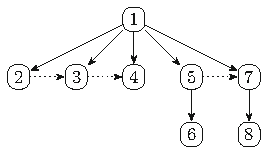
\includegraphics[width=.48\linewidth]{assets/front/dependencies.pdf}
\caption{章节之间的依赖关系. 实线箭头表示先修要求，虚线箭头表示引用关系.}\label{fig:front.1}
\end{figure}

每章最后都有一系列习题，让读者将所学概念用于正文没有讨论的问题.

\subsection*{致谢}\label{sec:acknowledgments}

\noindent\textbf{Sinho Chewi}\quad 最优传输并不是我读研究生时原本计划研究的方向，但它使我的科研生涯变得丰富得多. 为此，我感谢导师兼合作者Philippe，他勇于引领我进入这个美丽的领域；也感谢我的同门兼合作者Jon，他为我开辟道路，并不断给我灵感.

我对最优传输的理解来自许多来源，最初是Villani写作精湛的专著\cite{ref315}，还包括与合作者及Philippe课题组成员数不清的讨论时光. 我很高兴有机会通过这本教学著作为共同体的发展出一份力.

感谢高等研究院提供友好的工作环境，并通过Eric和Wendy Schmidt基金给予支持.

\noindent\textbf{Jonathan Niles-Weed}\quad 我很幸运能向许多才华横溢的合作者学习最优传输；其中，Jason Altschuler、Francis Bach、Sivaraman Balakrishnan、Quentin Berthet、Marco Cuturi、Vincent Divol、Alberto González-Sanz、Tudor Manole、Aram-Alexandre Pooladian、Austin Stromme与Larry Wasserman对我的影响尤其深远. 对他们的知识与见解，我深怀感激. 能在本书中分享他们的一些工作，是我的荣幸.

感谢2021年参加纽约大学研究生讨论班的学生，讨论班涉及本书部分内容，他们的反馈显著改善了表述. 我还要再次感谢Sivaraman Balakrishnan对本书早期版本提出的敏锐意见.

当然，若没有同事兼朋友Sinho Chewi与Philippe Rigollet，就不会有今天的我. 你们给我的启发难以衡量. 与你们合作是我职业生涯最精彩的经历之一，希望今后仍能有幸继续合作.

我在这些讲义上的工作主要由美国国家科学基金会CAREER奖DMS-2339829及其他若干NSF项目（DMS-2015291、DMS-2210583）支持，还得到Sloan基金会研究奖及Apple、Google的资助.

\noindent\textbf{Philippe Rigollet}\quad 自我有幸于2019年在圣弗卢尔开设系列讲座以来，这些讲义已经大幅扩充；最初讲座大致涵盖\autoref{sec:1}、\autoref{sec:7}和\autoref{sec:8}. 初次授课时，本书如今呈现的许多材料对我还很陌生.

首先，我衷心感谢2019年圣弗卢尔暑期学校的组织者，特别是Christophe Bahadoran，以及所有参与者. 听众提供的宝贵反馈，对促成这些讲义主题的大幅扩展起了关键作用. 我唯一的遗憾是成稿迟延，未能与出色的共同讲师Nicolas Curien和Elchanan Mossel的讲义同时出版. 尽管不能合为一卷，我们永远会以Chevaliers du Taste-fourme的身份相联.

我学到的大部分知识来自他人，感谢向我传授了许多这一主题知识的合作者：Jason Altschuler、Julien Clancy、Max Daniels、Aiden Forrow、Borjan Geshkovski、Florian Gunsilius、Jan-Christian Hütter、Cyril Letrouit、Jean-Michel Loubes、Chen Lu、Tyler Maunu、Mor Nitzan、Quentin Paris、Geoff Schiebinger、Austin Stromme、George Stepaniants、Felipe Suarez、William Torous、Kaizheng Wang、Yuling Yan和Aleksandr Zimin. 对于最优传输及其他主题上的启发性讨论，我还要特别感谢Sébastien Bubeck、Ramon van Handel、Thibaut Le Gouic、Vianney Perchet、Yury Polyanskiy、Maxim Raginsky和Justin Solomon. \autoref{sec:5}和\autoref{sec:6}中的许多思想是2021年秋伯克利Simons研究院“优化与抽样中的几何方法”项目的核心讨论话题. 感谢所有参与者、共同组织者及Peter Bartlett，使这一项目如此精彩而富有启发.

此后，统计最优传输共同体显著壮大，这些讲义也从与许多人的交流中受益. 从我们同在普林斯顿时把我引入最优传输的Marco Cuturi开始，我还从Guillaume Carlier、Victor Chernozhukov、Lenaïc Chizat、Simone Di Marino、Augusto Gerolin、Promit Ghosal、Marc Hallin、Zaid Harchaoui、Kengo Kato、Anna Korba、Alexei Kroshnin、Qin Li、Jan Maas、Axel Munk、Robert McCann、Dan Mikulincer、Youssef Marzouk、Soumik Pal、Victor Panaretos、Gabriel Peyré、Filippo Santambrogio、Bodhi Sen、Vladimir Spokoiny、Yair Shenfeld和Jia-Jie Zhu等人那里学到了许多最优传输知识.

部分材料曾于2023和2024年在麻省理工学院、2022年在巴黎索邦大学，以及2023年的两所暑期学校——普林斯顿机器学习理论暑期学校和意大利Cetraro的CIME暑期学校——讲授. 听众给予了出色反馈，促进讲义改进. 特别感谢Théo Dumont、Max Daniels和Giulia Bertagnolli分别录入相关材料.

Michael Diao、Haruki Kono、Hugo Lavenant、Aimee Maurais、Yaroslav Mukhin、Madhav Sankaranarayanan、Sabarish Sainathan、Yucheng Shang、Vishwak Srinivasan、Panos Tsimpos、Oliver Wang、Liane Xu和Julie Zhu纠正了一些排印错误与差错. 感谢他们帮助提高书稿的可读性.

最后，感谢出色的共同作者Sinho Chewi和Jonathan Niles-Weed. 谢谢你们与我一道踏上这场壮阔冒险. 我从你们身上学到的比从任何其他人身上都多；对我而言，你们既是学生，也同样是老师.

我在这些讲义上的工作主要获NSF项目CCF-1838071以及2019--2024年间的其他若干美国国家科学基金会项目（DMS-1712596、CCF-1740751、DMS-2022448、CCF-2106377）支持. 也感谢Apple的资助. 初稿构思于2019年春，当时我在高等研究院获Eric和Wendy Schmidt基金支持.

\noindent\textbf{利益冲突}\quad 作者声明，不存在与本书稿内容相关、需要披露的利益冲突.

\vspace{0.5cm}
\noindent\begin{tabular}{ll}
美国康涅狄格州纽黑文 & Sinho Chewi\\
纽约州纽约 & Jonathan Niles-Weed\\
美国马萨诸塞州剑桥 & Philippe Rigollet
\end{tabular}\par
\noindent 2024年7月
